\documentclass[12pt,openany]{book}
\usepackage{amsmath,amsthm,amsfonts,amscd} % Packages for mathematics
\usepackage{commath}
% Colors
\usepackage[dvipsnames, table]{xcolor}
\definecolor{titleblue}{RGB}{0,53,128}
\definecolor{chaptergray}{RGB}{140,140,140}
\definecolor{sectiongray}{RGB}{180,180,180}

\definecolor{thmcolor}{RGB}{231, 76, 60}
\definecolor{defcolor}{RGB}{52, 152, 219}
\definecolor{lemcolor}{RGB}{155, 89, 182}
\definecolor{corcolor}{RGB}{46, 204, 113}
\definecolor{procolor}{RGB}{241, 196, 15}
\definecolor{execolor}{RGB}{85, 123, 122}

% Fonts
\usepackage[T1]{fontenc}
\usepackage[utf8]{inputenc}
\usepackage{newpxtext,newpxmath}
\usepackage{sectsty}
\allsectionsfont{\sffamily\color{titleblue}\mdseries}

% Page layout
\usepackage{geometry}
\geometry{a4paper,left=.85in,right=.62in,top=1in,bottom=1in,heightrounded}
\usepackage{fancyhdr}
\fancyhf{}
\fancyhead[LE,RO]{\thepage}
\fancyhead[LO]{\nouppercase{\rightmark}}
\fancyhead[RE]{\nouppercase{\leftmark}}
\renewcommand{\headrulewidth}{0.5pt}
\renewcommand{\footrulewidth}{0pt}

% Chapter formatting
\usepackage{titlesec}
\titleformat{\chapter}[display]
{\normalfont\sffamily\Huge\bfseries\color{titleblue}}{\chaptertitlename\ \thechapter}{20pt}{\Huge}
\titleformat{\section}
{\normalfont\sffamily\Large\bfseries\color{titleblue!100!gray}}{\thesection}{1em}{}
\titleformat{\subsection}
{\normalfont\sffamily\large\bfseries\color{titleblue!75!gray}}{\thesubsection}{1em}{}

% Table of contents formatting
\usepackage{tocloft}
\renewcommand{\cftchapfont}{\sffamily\color{titleblue}\bfseries}
\renewcommand{\cftsecfont}{\sffamily\color{chaptergray}}
\renewcommand{\cftsubsecfont}{\sffamily\color{sectiongray}}
\renewcommand{\cftchapleader}{\cftdotfill{\cftdotsep}}

% Hyperlinks
\usepackage{hyperref}
\hypersetup{
	colorlinks=true,
	linkcolor=titleblue,
	filecolor=black,      
	urlcolor=titleblue,
}

%Listing
\usepackage{listings} %Code
\renewcommand{\lstlistingname}{Code}%

\definecolor{codegreen}{rgb}{0,0.6,0}
\definecolor{codegray}{rgb}{0.5,0.5,0.5}
\definecolor{codepurple}{rgb}{0.58,0,0.82}
\definecolor{backcolour}{rgb}{1,1,1}


\lstdefinestyle{sage}{
	language=Python,
	backgroundcolor=\color{white},
	basicstyle=\small\ttfamily\color{black}, 
	basicstyle=\footnotesize\ttfamily\color{black},
	keywordstyle=\color{blue!60!black},
	commentstyle=\color{green!60!black},
	stringstyle=\color{purple!60!black},
	showstringspaces=false,
	breaklines=true,
	tabsize=4,
	morekeywords={True, False, None},
	frame=leftline, % Remove the border
	framesep=3pt,
	frameround=tttt,
	framexleftmargin=3pt,
	numbers=left,
	numberstyle=\small\color{gray},
	xleftmargin=15pt, % Increase the left margin
	xrightmargin=5pt,
	captionpos=b,
	belowskip=0pt,
	aboveskip=4pt
}

%Ceiling and Floor Function
\usepackage{mathtools}
\DeclarePairedDelimiter{\ceil}{\lceil}{\rceil}
\DeclarePairedDelimiter{\floor}{\lfloor}{\rfloor}

%Algorithm
\usepackage[ruled,linesnumbered]{algorithm2e}
\usepackage{setspace}
\usepackage{algpseudocode}
\SetKwComment{Comment}{/* }{ */}
\SetKw{Break}{break}
\SetKw{Downto}{downto}
\SetKwProg{Fn}{Function}{:}{end}
\SetKwFunction{KeyGens}{KeyGens}

\renewcommand{\arraystretch}{1.25}
%---------------------------My Preamble
\usepackage{marvosym} %Lightning
\usepackage{booktabs}
\usepackage{multicol}
\setlength{\columnsep}{2cm}
\setlength{\columnseprule}{1.25pt}
\usepackage{enumerate}
\usepackage{soul}
\newcommand{\mathcolorbox}[2]{\colorbox{#1}{$\displaystyle #2$}}
\usepackage{graphicx}
\usepackage{tikz}
\usepackage{tikz-cd}
\usetikzlibrary{calc}
\usetikzlibrary{arrows, arrows.meta, positioning, shapes, shapes.multipart}
\usepackage{pgfplots}
\pgfplotsset{compat=1.16}
\usepackage{caption}

%Tcolorbox
\usepackage[most]{tcolorbox}
\tcbset{colback=white, arc=5pt}
%\tcbset{enhanced, colback=white,colframe=black,fonttitle=\bfseries,arc=4mm,boxrule=1pt,shadow={2mm}{-1mm}{0mm}{black!50}}
%White box with black text and shadow
%\begin{tcolorbox}[colback=white,colframe=black,fonttitle=\bfseries,title=Black Shadow Box,arc=4mm,boxrule=1pt,shadow={2mm}{-1mm}{0mm}{black!50}]
%	This is a white box with black text and a subtle shadow. The shadow adds some depth and dimension to the box without overpowering the design.
%\end{tcolorbox}

%Theorem
\newtheorem{axiom}{Axiom}[chapter]
\newtheorem{theorem}{Theorem}[chapter]
\newtheorem{proposition}[theorem]{Proposition}
\newtheorem{corollary}{Corollary}[theorem]
\newtheorem{lemma}[theorem]{Lemma}

\theoremstyle{definition}
\newtheorem{definition}{Definition}[chapter]
\newtheorem{construction}{Construction}[chapter]
\newtheorem{remark}{Remark}[chapter]
\newtheorem{exercise}{Exercise}[chapter]
\newtheorem{example}{Example}[chapter]
\newtheorem*{note}{Note}

%New Command
\newcommand{\N}{\mathbb{N}}
\newcommand{\Z}{\mathbb{Z}}
\newcommand{\Q}{\mathbb{Q}}
\newcommand{\R}{\mathbb{R}}
\newcommand{\C}{\mathbb{C}}
\newcommand{\F}{\mathbb{F}}
\newcommand{\G}{\mathbb{G}}

\newcommand{\img}{\operatorname{\textnormal{Img}}}
\newcommand{\id}{\operatorname{\textnormal{Id}}}

\newcommand{\inv}[1]{#1^{-1}}

\newcommand{\ie}{\textnormal{i.e.}}
\newcommand{\eg}{\textnormal{e.g.}}

\newcommand{\of}[1]{\left( #1 \right)} 
\renewcommand{\abs}[1]{\left\lvert #1 \right\rvert}
\renewcommand{\norm}[1]{\left\| #1 \right\|}

\newcommand{\sol}{\textcolor{magenta}{\bf Solution}}

\newcommand{\KeyGen}{\mathsf{KeyGen}}
\newcommand{\Enc}{\mathsf{Enc}}
\newcommand{\Dec}{\mathsf{Dec}}
\newcommand{\scheme}{\Sigma}
\newcommand{\keyspace}{\mathcal{K}}
\newcommand{\messagespace}{\mathcal{M}}
\newcommand{\ciphertextspace}{\mathcal{C}}

\newcommand{\library}{\mathcal{L}}
\newcommand{\zero}{\textcolor{red}{\texttt{0}}}
\newcommand{\one}{\textcolor{red}{\texttt{1}}}

\newcommand{\tab}{\hspace{12pt}}
\newcommand{\xor}{\oplus}
\newcommand{\adversary}{\mathcal{A}}
\newcommand{\isequal}{\overset{?}{=}}
\newcommand{\linking}{\diamond}

\newcommand{\true}{\texttt{true}}
\newcommand{\false}{\texttt{false}}
\newcommand{\randomness}{\$}
\newcommand{\uniform}{\xleftarrow{\randomness}}
\newcommand{\binaryfield}{\set{\zero,\one}}

\newcommand{\ctxt}{\texttt{CTXT}}
\newcommand{\eavesdrop}{\texttt{Eavesdrop}}

\newcommand{\ots}{\mathsf{ots}}
\newcommand{\sL}{\mathsf{L}}
\newcommand{\sR}{\mathsf{R}}

\newcommand*{\indist}{%
	\mathrel{\vcenter{\offinterlineskip
			\hbox{$\sim$}\vskip-.35ex\hbox{$\sim$}\vskip-.35ex\hbox{$\sim$}}}}

\newcommand{\outputs}{\Rightarrow}

% Begin document
\begin{document}
	
	% Title page
	\begin{titlepage}
		\begin{center}
			{\Huge\textsf{\textbf{Code-Based Games Philosophy}}\par}
			\vspace{0.5in}
			{\Large Ji Yong-Hyeon, Kim Dong-Hyeon\par}
			\vspace{1in}
			%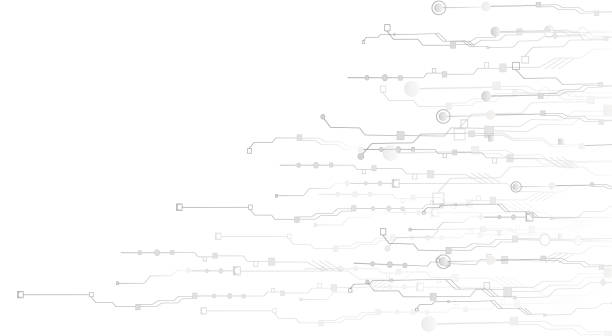
\includegraphics[scale=2.5]{urop.jpg}\par
			\begin{figure}[h!]\centering
				\begin{tikzpicture}[node distance=3cm]
					
					% Define block styles
					\tikzstyle{decision} = [diamond, draw, fill=pink!30, 
					text width=4.5em, text badly centered, inner sep=0pt]
					\tikzstyle{block} = [rectangle, draw, fill=cyan!30, 
					text width=5em, text centered, rounded corners, minimum height=4em]
					\tikzstyle{line} = [draw, -latex', color=gray!70]
					
					% Nodes
					\node [block] (init) {Start};
					\node [decision, right of=init] (decide) {Choose b $\in$ \{0,1\}};
					\node [block, above right of=decide, node distance=3cm] (game0) {$\mathcal{E}_0$};
					\node [block, below right of=decide, node distance=3cm] (game1) {$\mathcal{E}_1$};
					\node [block, right of=decide, node distance=4cm] (output) {Output to adversary};
					\node [decision, right of=output] (adversary) {Adversary's guess b'};
					\node [block, right of=adversary] (end) {Win if $b = b'$};
					
					% Paths
					\path [line] (init) -- (decide);
					\path [line] (decide) |- (game0);
					\path [line] (decide) |- (game1);
					\path [line] (game0) -| (output);
					\path [line] (game1) -| (output);
					\path [line] (output) -- (adversary);
					\path [line] (adversary) -- (end);
				\end{tikzpicture}
			\end{figure}
			\vspace{1in}
			{\bf Department of Information Security, Cryptology, and Mathematics\par}
			{College of Science and Technology\par}
			{Kookmin University\par}
			%
\includegraphics[width=1.5in]{school_logo.jpg}\par
			\vspace{.25in}
			{\large \today\par}
		\end{center}
	\end{titlepage}
	
	% Table of contents
	\tableofcontents
	
	% Chapters
	\mainmatter
	
	\chapter*{List of Symbols}
	
	\begin{tabular}{ll}
		\( \zero^\lambda, \one^\lambda\) & \(\underbrace{\zero\zero\cdots\zero}_{\lambda\ \text{times}}, \underbrace{\one\one\cdots\one}_{\lambda\ \text{times}}\) : \(\lambda\)-bit zero/one sequence \\
		\( \adversary\linking\library \) & The result of \textbf{linking} $\adversary$ to  $\library$ \\
		\( \randomness \) & Randomeness \\
		\( \equiv \) & Interchangability; Identical
	\end{tabular}
	
	\chapter{One-Time Pad \& Kerckhoff's Principle}
	
	\begin{tcolorbox}[colback=white,colframe=magenta,arc=5pt,title={\color{white}\bf }]
		\textbf{Kerchkhoffs' Principle:}
		\begin{quote}
			Design your system to be secure even if the attacker has complete knowledge of all its algorithms.
		\end{quote}
	\end{tcolorbox}
	\vspace{8pt}
	\begin{tcolorbox}[colback=white,colframe=defcolor,arc=5pt,title={\color{white}\bf One-time Pad (OTP)}]
		\begin{construction}
			The specific \(\KeyGen,\Enc\), and \(\Dec\) algorithms for \textbf{one-time pad} are given below: \begin{center}
				\begin{tabular}{|lll|}
					\hline
					$\underline{\KeyGen:}$ & \(\underline{\Enc(k,m\in\binaryfield^\lambda):}\) & \(\underline{\Dec(k,c\in\binaryfield^\lambda):}\)\\
					\tab$k\uniform\binaryfield^\lambda$ & \tab return \(k\xor m\) & \tab return \(k\xor c\)\\
					\tab return $k$ &&\\
					\hline
				\end{tabular}\\
			\end{center}
		\end{construction}
	\end{tcolorbox}
	\vspace{8pt}
	\begin{tcolorbox}[colback=white,colframe=procolor,arc=5pt,title={\color{white}\bf Corectness of OTP}]
		\begin{proposition}
			\[
			(\forall k,m\in\binaryfield^\lambda)\quad\Dec(k,\Enc(k,m))=m.
			\]
		\end{proposition}
	\end{tcolorbox}
	\begin{proof}
		Let \(k,m\in\binaryfield^\lambda\) then \begin{align*}
			\Dec(k,\Enc(k,m))=\Dec(k,k\xor m)&=k\xor(k\xor m)\\
			&=(k\xor k)\xor m\\
			&=\zero^\lambda\xor m\\
			&=m.
		\end{align*}
	\end{proof}

	\newpage
	\begin{remark}[\eavesdrop\ Algorithm]
		From Eve’s perspective, seeing a ciphertext corresponds to receiving
		an output from the following algorithm: \\ \begin{center}
		\begin{tabular}{|l|}
			\hline
			\(\underline{\eavesdrop(m\in\binaryfield^\lambda)}\)\\
			\tab\(k\uniform\binaryfield^\lambda\)\\
			\tab\(c:=k\xor m\)\\
			\tab return \(c\)\\
			\hline
		\end{tabular}
		\end{center}
	\end{remark}

	\begin{tcolorbox}[colback=white,colframe=thmcolor,arc=5pt,title={\color{white}\bf }]
		\begin{theorem}
			Let \(m\in\binaryfield^\lambda\). The distribution \(\eavesdrop(m)\) is the \textbf{uniform distribution} on \(\binaryfield^\lambda\). In other words, \[
			m,m'\in\binaryfield^\lambda\implies\textnormal{dist}(\eavesdrop(m))\sim\textnormal{dist}(\eavesdrop(m')).
			\]
		\end{theorem}
	\end{tcolorbox}
	\begin{proof}
		content...
	\end{proof}
	
	\chapter{The Basics of Provable Security}
	
	\section{How to Write a Security Definition}
	\subsection{Syntax and Correctness}
	
	\begin{tcolorbox}[colback=white,colframe=defcolor,arc=5pt,title={\color{white}\bf Encryption Syntax}]
		\begin{definition}
			A \textbf{symmetric-key encryption (SKE) scheme} consists of the following algorithms: \begin{itemize}
				\item $\KeyGen$ outputs a key $k=\KeyGen(1^\lambda)\in\keyspace$
				\item $\Enc:\keyspace\times\messagespace\to\ciphertextspace$
				\item $\Dec:\keyspace\times\ciphertextspace\to\messagespace$
			\end{itemize} We call $\keyspace$ the \textbf{key space}, $\messagespace$ the \textbf{message space}, and $\ciphertextspace$ the \textbf{ciphertext space} of the scheme.
		\end{definition}
	\end{tcolorbox}
	\begin{remark}
		Note that \begin{itemize}
			\item \(\KeyGen\) is a randomized algorithm\footnote{An algorithm that makes use of random numbers.}.
			\item \(\Enc\) is a (possibly randomized) algorithm\footnote{It could operate deterministically or non-deterministically depending on specific conditions or parameters.}.
			\item \(\Dec\) is a deterministic algorithm\footnote{An algorithm that does produces the same output for the same input, every time it's run.}.
		\end{itemize}
	\end{remark}
	\begin{remark}
		We refer to the entire scheme by a single variable $\scheme$, \ie, $$
		\scheme=(\KeyGen, \Enc, \Dec).
		$$
	\end{remark}
	\begin{remark}
		We write \[
		\begin{array}{ccc}
			\scheme.\KeyGen, & \scheme.\Enc, & \scheme.\Dec,\\
			\scheme.\keyspace, & \scheme.\messagespace, &\scheme.\ciphertextspace
		\end{array}
		\] to refer to its components.
	\end{remark}
	\vspace{8pt}
	\begin{tcolorbox}[colback=white,colframe=defcolor,arc=5pt,title={\color{white}\bf SKE Correctness}]
		\begin{definition}
			An encryption scheme $\scheme$ satisfies \textbf{correctness} if \[
			\left(\forall k\in\scheme.\keyspace\right)\left(\forall m\in\scheme.\messagespace
			\right)\quad\Pr\left[\scheme.\Dec(k, \scheme.\Enc(k,m))=m\right]=1.
			\]
		\end{definition}
	\end{tcolorbox}
	\begin{remark}
		The definition is written in terms of a probability because $\Enc$ is allowed to be a randomized algorithm. In other words, decrypting a ciphertext with the same key that was used for encryption must \textit{always} result in the original plaintext.
	\end{remark}
	\vspace{4pt}
	\begin{example}
		content...
	\end{example}
	
	\subsection{``Real-vs-Random'' Style of Security Definition}
	\begin{quote}
		``an encryption scheme is a good one if its ciphertexts \textit{look like} random junk to an attacker''
	\end{quote}

	Security definitions always consider \textbf{the attacker's view} of the system.
	\begin{quote}
		``an encryption scheme is a good one if its ciphertexts \textit{look like} random junk to an attacker ... when each key is secret and used to encrypt only one plaintext, even when the attacker chooses the plaintexts.''
	\end{quote}

	
	A concise way to express all of these details is to consider \textbf{the attacker as a calling	program} to the following subroutine:
	\begin{center}
		\begin{tabular}{|l|}
			\hline
			$\underline{\texttt{CTXT}(m\in\scheme.\messagespace):}$\\
			\tab$k\gets\scheme.\KeyGen$\\
			\tab$c:=\scheme.\Enc(k,m)$\\
			\tab return $c$\\
			\hline
		\end{tabular}\\
	\end{center}
	
	\begin{example}[One-Time Pad (OTP)]
		a\\ \begin{center}
			\begin{minipage}{.44\textwidth}
				\begin{tabular}{|l|}
					\hline
					$\underline{\texttt{CTXT}(m):}$\\
					\begin{tabular}{ll}
						\tab$k\gets\binaryfield^\lambda$ & \textcolor{gray}{//\(\KeyGen\) of OTP}\\
						\tab$c:=k\xor m$ & \textcolor{gray}{//\(\Enc\) of OTP}\\
						\tab return $c$\\
					\end{tabular}\\
					\hline
				\end{tabular}\\
			\end{minipage} vs.
		\begin{minipage}{.3\textwidth}
			\begin{tabular}{|l|}
				\hline
				$\underline{\texttt{CTXT}(m):}$\\
				\begin{tabular}{ll}
					\tab$c:=\binaryfield^\lambda$ & \textcolor{gray}{//\(\ciphertextspace\) of OTP}\\
					\tab return $c$\\
				\end{tabular}\\
				\hline
			\end{tabular}\\
		\end{minipage}
		\end{center}
	\end{example}

	\begin{quote}
		``an encryption scheme is a good one if, when you plug its \(\KeyGen\) and \(\Enc\) algorithms into the template of the \texttt{CTXT} subroutine above, the two implementations of \texttt{CTXT} induce identical behavior in every calling program.''
	\end{quote}

	\subsection{``Left-vs-Right'' Style of Security Definition}
	
	\section{Formalisms for Security Definition}
	\begin{tcolorbox}[colback=white,colframe=defcolor,arc=5pt,title={\color{white}\bf Library}]
		\begin{definition}
			A \textbf{library} $\library$ is a collection of subroutines and private/static variables.
		\end{definition}
	\end{tcolorbox}
	\begin{example}
		Here is a familiar library and one possible calling program:
		\begin{center}
			\begin{minipage}{.25\textwidth}
				\begin{tabular}{|c|}
					\hline
					\cellcolor{blue!25}$\library$\\
					\hline
					\begin{tabular}{l}
						\underline{\texttt{CTXT}($m$):}\\
						\tab $k\uniform\set{\zero, \one}^\lambda$\\
						\tab $c:=k\xor m$\\
						\tab return $c$
					\end{tabular}\\
					\hline
				\end{tabular}\quad,\quad
			\end{minipage}
			\begin{minipage}{.25\textwidth}
				\begin{tabular}{|c|}
					\hline
					\cellcolor{blue!25}$\adversary$\\
					\hline
					\begin{tabular}{l}
						$m\gets\set{\zero,\one}^\lambda$\\
						$c:=\texttt{CTXT}(m)$\\
						return $m\isequal c$
					\end{tabular}\\
					\hline
				\end{tabular}
			\end{minipage}.
		\end{center} Then \[
		\Pr\left[\adversary\linking\library\Rightarrow\true\right]=\frac{1}{2^\lambda}.
		\]
	\end{example}
	\vspace{8pt}
	\begin{tcolorbox}[colback=white,colframe=defcolor,arc=5pt,title={\color{white}\bf Interchangeability}]
		\begin{definition}
			Let $\library_1$ and $\library_2$ be two libraries that have the same interface. We say that $\library_1$ and $\library_2$ are \textbf{interchangeable}, and write $\library_1\equiv\library_2$, if $\forall\adversary:$\[
			\Pr\left[\adversary\linking\library_1\Rightarrow\true\right]=
			\Pr\left[\adversary\linking\library_2\Rightarrow\true\right].
			\]
		\end{definition}
	\end{tcolorbox}
	\vspace{8pt}

	\begin{tcolorbox}[colback=white,colframe=defcolor,arc=5pt,title={\color{white}\bf One-Time Uniform Ctxts}]
		\begin{definition}
			An encryption scheme $\scheme$ has \textbf{one-time uniform cipher-texts} if 
			\begin{center}
				\begin{minipage}{.3\textwidth}
					\begin{tabular}{|c|}
						\hline
						\cellcolor{blue!25}$\library_{\text{ots\$-real}}^\scheme$\\
						\hline
						\begin{tabular}{l}
							\underline{\texttt{CTXT}($m\in\scheme.\messagespace$):}\\
							\tab $k\gets\scheme.\KeyGen$\\
							\tab $c\gets\scheme.\Enc(k,m)$\\
							\tab return $c$
						\end{tabular}\\
						\hline
					\end{tabular}
				\end{minipage}
				$\equiv$\quad
				\begin{minipage}{.3\textwidth}
					\begin{tabular}{|c|}
						\hline
						\cellcolor{blue!25}$\library_{\text{ots\$-rand}}^\scheme$\\
						\hline
						\begin{tabular}{l}
							\underline{\texttt{CTXT}($m\in\scheme.\messagespace$)}:\\
							\tab $c\gets\scheme.\ciphertextspace$\\
							\tab return $c$
						\end{tabular}\\
						\hline
					\end{tabular}
				\end{minipage}
			\end{center}
		\end{definition}
	\end{tcolorbox}

	\begin{tcolorbox}[colback=white,colframe=defcolor,arc=5pt,title={\color{white}\bf One-Time Secrecy (\(\mathsf{OTS})\)}]
		\begin{definition}\textbf{
			One-time secrecy} is a property of an encryption scheme where an adversary cannot gain any information about the plaintext message from the ciphertext, even if they know the encryption key was used only once.
			\begin{center}
				\begin{minipage}{.3\textwidth}
					\begin{tabular}{|c|}
						\hline
						\cellcolor{blue!25}$\library_{\ots-\sL}^\scheme$\\
						\hline
						\begin{tabular}{l}
							\underline{\texttt{Eve}($m_L,m_R\in\scheme.\messagespace$):}\\
							\tab $k\gets\scheme.\KeyGen$\\
							\tab $c\gets\scheme.\Enc(k,m_L)$\\
							\tab return $c$
						\end{tabular}\\
						\hline
					\end{tabular}
				\end{minipage}
				$\equiv$
				\begin{minipage}{.3\textwidth}
					\begin{tabular}{|c|}
						\hline
						\cellcolor{blue!25}$\library_{\ots-\sR}^\scheme$\\
						\hline
						\begin{tabular}{l}
							\underline{\texttt{Eve}($m_L,m_R\in\scheme.\messagespace$):}\\
							\tab $k\gets\scheme.\KeyGen$\\
							\tab $c\gets\scheme.\Enc(k,m_R)$\\
							\tab return $c$
						\end{tabular}\\
						\hline
					\end{tabular}
				\end{minipage}
			\end{center}
		\end{definition}
	\end{tcolorbox}
	
	\section{How to Demonstrate Insecurity with Attacks}
	\section{How to Prove Security with The Hybrid Technique}
	\section{How to Compare/Contract Security Definitions}
	
	\newpage
	\section*{Exercises}
	\begin{tcolorbox}[colback=white,colframe=execolor,arc=5pt,title={\color{white}\bf }]
		\begin{exercise}
			In abstract algebra, a (finite) group is a finite set $\mathbb{G}$ of items together with an operator $\otimes$ satisfying the following axioms:
			\begin{itemize}
				\item \textbf{Closure:} for all \(a,b\in\mathbb{G}\), we have $a\otimes b\in \mathbb{G}$
				\item \textbf{Identity:} there is a special \textit{identity element} $e\in\G$ that satisfies \(e\otimes a = a\otimes e = a\) for
				all \(a\in\G\). We typically write ``1'' rather than $e$ for the identity element.
				\item \textbf{Associativity:} for all \(a, b, c\in\G\), we have \((a\otimes b)\otimes c = a\otimes (b\otimes c)\).
				\item \textbf{Inverses:} for all \(a\in\G\), there exists an inverse element \(b\in\G\) such that \(a\otimes b = b\otimes a\)
				is the identity element of $\G$. We typically write ``$a^{-1}$'' for the inverse of $a$.
			\end{itemize}
			
			Define the following encryption scheme in terms of an arbitrary group \((\G, \otimes)\):
			\begin{center}
				\begin{tabular}{|clll|}
					\hline
					\(\keyspace=\G\) & \(\underline{\KeyGen:}\) & \(\underline{\Enc(k,m):}\) &\(\underline{\Dec(k,c):}\) \\
					\(\messagespace=\G\) & \tab\(k\gets\G\) & \tab return \(k\otimes m\) & \tab ??\\
					\(\ciphertextspace=\G\) & \tab return \(k\) &&\\
					\hline
				\end{tabular}
			\end{center}
			\begin{enumerate}[(a)]
				\item Prove that \(\binaryfield^\lambda\) is a group with respect to the xor operator. What is the identity
				element, and what is the inverse of a value $x\in\binaryfield^\lambda$?
				\item Fill in the details of the $\Dec$ algorithm and prove (using the group axioms) that the scheme satisfies correctness.
				\item Prove that the scheme satisfies one-time secrecy.
			\end{enumerate}
		\end{exercise}
	\end{tcolorbox}
	\iffalse
	\begin{proof}[\sol]
		\begin{enumerate}[(a)]
			\item We show that \((\binaryfield^\lambda,\xor)\) satisfies the group axioms:
			\begin{itemize}
				\item[] \textbf{Closure:} \(x,y\in\binaryfield^\lambda\implies x\xor y\in\binaryfield^\lambda\)
				\item[] \textbf{Associativity:} The XOR operation is associative, so this property holds.
				\item[] \textbf{Identity:} The identity for XOR is the all-zero \(\lambda\)-bit string \(\zero^\lambda\) because \[
				(\forall x\in\binaryfield^\lambda)\quad x\xor\zero^\lambda=\zero^\lambda\xor x= x.
				\]
				\item[] \textbf{Inverse:} The inverse of $x$ under XOR is $x$ itself because \[
				x\xor x=\zero^\lambda.
				\]
			\end{itemize}
			\vspace{4pt}
			\item Decryption Algorithm: \begin{center}
				\begin{tabular}{l}
					\(\underline{\Dec(k,c):}\) \\ \tab return \(\inv{k}\otimes c\)
				\end{tabular}
			\end{center}
			Proof of Correctness: \begin{align*}
				\Dec(k,\Enc(k,m))&=\inv{k}\otimes\Enc(k,m)\\
				&=\inv{k}\otimes(k\otimes m)\\
				&=(\inv{k}\otimes k)\otimes m\\
				&=1\otimes m\\
				&=m.
			\end{align*}
			\item Let $m_L,m_R\in\G$ with $m_L\neq m_R$, and let $k\in\G$. The ciphertexts for theses message are \begin{align*}
				&c_L:=m_L\otimes k,\\
				&c_R:=m_R\otimes k.
			\end{align*} Let $\G:=\binaryfield^\lambda$ and $\otimes:=\xor$. Then \begin{align*}
				c_L\otimes c_R&=(m_L\otimes k)\otimes(m_R\otimes k)\\
				&=m_L\otimes m_R\otimes(k\otimes k)\\
				&=m_L\otimes m_R.
			\end{align*} This result does not reveal any information about $k$, and it would be the same if the attacker knew $m_L$ and $m_R$ but did not know $k$. Therefore, the scheme satisfies one-time secrecy.
			
			Note that if $\G=\binaryfield^\lambda$ and $\otimes=\xor$ then
			\begin{center}
				\begin{minipage}{.46\textwidth}
					\begin{tabular}{|c|}
						\hline
						\cellcolor{blue!25}$\library_{\ots-\sL}^\scheme$ \\
						\hline
						\begin{tabular}{l}
							\underline{\texttt{Eve}($m_L,m_R\in\G$):}\\
							\tab $k\gets\G$\quad\textcolor{gray}{//\(\scheme.\KeyGen\)}\\
							\tab $c\gets k\otimes m_L$\quad\textcolor{gray}{//\(\scheme.\Enc(k,m_L)\)}\\
							\tab return $c$
						\end{tabular}\\
						\hline
					\end{tabular}
				\end{minipage}$\equiv$
				\begin{minipage}{.46\textwidth}
					\begin{tabular}{|c|}
						\hline
						\cellcolor{blue!25}$\library_{\ots-\sR}^\scheme$ \\
						\hline
						\begin{tabular}{l}
							\underline{\texttt{Eve}($m_L,m_R\in\G$):}\\
							\tab $k\gets\G$\quad\textcolor{gray}{//\(\scheme.\KeyGen\)}\\
							\tab $c\gets k\otimes m_R$\quad\textcolor{gray}{//\(\scheme.\Enc(k,m_R)\)}\\
							\tab return $c$
						\end{tabular}\\
						\hline
					\end{tabular}
				\end{minipage}
			\end{center}
		\end{enumerate}
	\end{proof}
	\fi
	\vspace{20pt}
	\begin{tcolorbox}[colback=white,colframe=execolor,arc=5pt,title={\color{white}\bf }]
		\begin{exercise}
			Prove that if an encryption scheme $\scheme$ has $\abs{\scheme.\keyspace}<\abs{\scheme.\messagespace}$ then it cannot satisfy one-time secrecy.\\
			\\
			\textcolor{gray}{[Hint: The definition of interchangeability does not place any restriction on the running time of the distinguisher/calling program. Even an exhaustive brute-force attack would be valid]}
		\end{exercise}
	\end{tcolorbox}
	\begin{proof}[\sol]
		content...
	\end{proof}

	\newpage
	\chapter{Cryptography on Intractable Computations}
	
	
	\section{What Qualifies as a ``Computationally Infeasible'' Attack?}
	\begin{tcolorbox}[colframe=defcolor,title={\color{white}\bf Polynomial Time}]
		\begin{definition}
			A program runs in \textbf{polynomial time} if \[
			\exists c>0:\forall n\geq n_0:\mathsf{Time}(n)\leq n^c,
			\] where \(\mathsf{Time}\) is the time taken by the algorithm on inputs of size \(n\). \(n_0\) is constant size of  the input. That is, there exists a constant $c > 0$ such that for all sufficiently long input strings $x$ with $\abs{x}=n$, the program stops after no more than $O(n^c)$ steps.
		\end{definition}
	\end{tcolorbox}
	\begin{remark}
		We see ``\textcolor{blue}{polynomial-time}'' as a synonym for ``\textcolor{blue}{efficient}.''
	\end{remark}
	\vspace{10pt}
	\begin{example}
		\(\gcd(a,b)\) can be computed using \(O((\log_2a)^3)\) bit operation if \(a>b\).
	\end{example}
	\vspace{10pt}
	\begin{example}
		\ \begin{table}[h!]\centering
			\begin{tabular}{l|l}
				\textbf{Efficient algorithm known:} & \textbf{No known efficient algorithm:}\\
				Computing GCDs & Factoring integers\\
				Arithmetic \(\bmod N\) & Computing \(\phi(N)\) given \(N\) \\
				Inverses \(\bmod N\) & Discrete logarithm \\
				Exponentiation \(\bmod N\) & Square roots \(\bmod\) composite \(N\) \\
			\end{tabular}
		\end{table}
	
		Again, ``efficient'' means polynomial-time. Furthermore, we only consider polynomial-time algorithms that run on standard, \textit{classical} computers. In fact, all of the problems in the right-hand column \textit{do} have known polynomial-time algorithms on \textit{quantum} computers.
	\end{example}
	\newpage
	\section{What Qualifies as a ``Negligible'' Success Probability?}
	For a cryptographic system to be considered secure, we often want the success probability of any polynomial-time adversary to be negligible in the security parameter \(\lambda\).  
	\vspace{8pt}
	\begin{tcolorbox}
		\textbf{Idea.}\tab \(\displaystyle\frac{1}{2^\lambda}\) \textbf{approaches zero so fast that no polynomial can ``rescue''}.
	\end{tcolorbox}
	
	\begin{proof}
		Assume that \(f(\lambda)=\frac{1}{2^\lambda}\). \begin{center}
			\begin{tikzpicture}[scale=.9]
				\begin{axis}[
					axis lines = left,
					xlabel = \(\lambda\),
					ylabel = \(f\),
					ymin = 0, ymax = 1.1,
					xmin = 0, xmax = 10,
					]
					\addplot [
					line width=.7mm,
					domain=0:10, 
					samples=100, 
					color=red,
					]
					{1/2^x};
					\addlegendentry{\(\frac{1}{2^\lambda}\)}
				\end{axis}
			\end{tikzpicture}
		\end{center} Consider any polynomial \(p(\lambda)\) of degree \(n\), written as: \[
		p(\lambda)=a_0+a_1\lambda+a_2\lambda^2+\cdots+a_n\lambda^n=\sum_{i=0}^{n}a_i\lambda^i.
		\] The product \(p(\lambda)\) and \(f(\lambda)\) is \[
		p(\lambda)f(\lambda)=a_0\frac{1}{2^\lambda}+a_1\frac{\lambda}{2^\lambda}+\cdots+a_n\frac{\lambda^n}{2^\lambda}.
		\] We claim that $\displaystyle
		\lim\limits_{\lambda\to\infty}a_k\frac{\lambda^k}{2^\lambda}=0,
		$ where \(k\in\Z_{\geq 0}\). Let \(g(\lambda)=\lambda^k\) and \(h(\lambda)=2^\lambda\). Note that 
		\begin{align*}
			h'(\lambda)=2^\lambda(\ln 2),\quad &g'(\lambda)=k\lambda^{k-1}\\
			h''(\lambda)=2^\lambda(\ln 2)^2,\quad &g''(\lambda)=k(k-1)\lambda^{k-2}\\
			&\vdots\\
			h^{(k)}(\lambda)=2^\lambda(\ln 2)^k,\quad&g^{(k)}(\lambda)=k!.
		\end{align*} By applying L'H\^{o}pital's Rule \(k\) times, we have \[
		\lim\limits_{\lambda\to\infty}\frac{\lambda^k}{2^\lambda}=\lim\limits_{\lambda\to\infty}\frac{k!}{2^\lambda(\ln 2)^k}=0.
		\] Thus, \(\lim\limits_{\lambda\to\infty}p(\lambda)f(\lambda)=0\).
	\end{proof}
	\begin{tcolorbox}[colframe=defcolor,title={\color{white}\bf Negligible}]
		\begin{definition}
			A function \(f\) is \textbf{negligible} if, \[
			\forall\text{polynomial}\ p:\lim\limits_{\lambda\to\infty}p(\lambda)f(\lambda)=0.
			\] In other words, a negligible function approaches zero so fast that you can never catch up when mutiplying by a polynomial.
		\end{definition}
	\end{tcolorbox}
	\begin{remark}
		As $\textcolor{blue}{\lambda}$ (\textcolor{blue}{security parameter}) gets larger and larger, the product of \(\textcolor{blue}{p(\lambda)}\) (\textcolor{blue}{resources or capabilities for an adversary}) and \(\textcolor{blue}{f(\lambda)}\) (\textcolor{blue}{success probability}) approaches \(0\).
	\end{remark}
	\begin{remark}
		A function $f(\lambda)$ is negligible if $\forall p(\lambda)> 0:\exists\lambda_0:\lambda>\lambda_0\Rightarrow \abs{f(\lambda)}<\frac{1}{p(\lambda)}$.
	\end{remark}
	\vspace{8pt}
	\begin{tcolorbox}[colframe=procolor,title={\color{white}\bf }]
		\begin{proposition}
			Let \(c\in\Z\). \[
			\lim\limits_{\lambda\to\infty}\lambda^cf(\lambda)=0\implies\text{$f$ is negligible}.
			\]
		\end{proposition}
	\end{tcolorbox}
	\begin{proof}
		Suppose that \(f\) satisfies \(\lim\limits_{\lambda\to\infty}\lambda^c f(\lambda)=0\) for any \(c\in\Z\), and take an arbitrary polynomial \(p\) of degree \(n\). Since \(\lim\limits_{\lambda\to\infty}\frac{p(\lambda)}{\lambda^{n+1}}=0\), we have \[
		\lim\limits_{\lambda\to\infty}p(\lambda)f(\lambda)=\lim\limits_{\lambda\to\infty}\left[\frac{p(\lambda)}{\lambda^{n+1}}\left(\lambda^{n+1}\cdot f(\lambda)\right)\right]=\left(\lim\limits_{\lambda\to\infty}\frac{p(\lambda)}{\lambda^{n+1}}\right)\left(\lim\limits_{\lambda\to\infty}\lambda^{n+1} f(\lambda)\right) = 0\cdot 0=0.
		\]
	\end{proof}
	\vspace{8pt}
	\begin{example}
		Let \(c\in\Z\). Then \[
		\lim\limits_{\lambda\to\infty}\lambda^c\frac{1}{2^\lambda}=
		\lim\limits_{\lambda\to\infty}\frac{(\lambda^c)^{\log_2 2}}{2^\lambda}=
		\lim\limits_{\lambda\to\infty}\frac{2^{c\log_2\lambda}}{2^\lambda}=
		\lim\limits_{\lambda\to\infty}2^{c\log_2(\lambda)-\lambda}=0
		\] since \(c\log_2(\lambda)-\lambda\to-\infty\) as \(\lambda\to\infty\).
		 Thus, \(1/2^\lambda\) is negligible.
	\end{example}

	\begin{tcolorbox}[colframe=defcolor,title={\color{white}\bf \(f\approx g\)}]
		\begin{definition}
			Let \(f,g:\N\to\R\) are real-valued functions. We write \(f\approx g\) to mean that \(\abs{f(\lambda)-g(\lambda)}\) is a negligible function.
		\end{definition}
	\end{tcolorbox}

	\begin{remark}
		We use the terminology of negligible functions exclusively when discussing probabilities, so the following are common: \begin{align*}
			\Pr[X]\approx 0 &\Leftrightarrow \text{``event $X$ almost never happens''}\\
			\Pr[Y]\approx 1 &\Leftrightarrow \text{``event $Y$ almost always happens''}\\
			\Pr[A]\approx \Pr[B] &\Leftrightarrow \text{``event $A$ and $B$ happen with essentially the same probability''}
		\end{align*}
		Additionally, the \(\approx\) symbol is \textit{transitive}: \[
		\Pr[X]\approx\Pr[Y]\land\Pr[Y]\approx\Pr[Z]\implies\Pr[X]\approx\Pr[Z].
		\]
	\end{remark}

	\newpage
	\section{Indistinguishability}
	\begin{tcolorbox}[colframe=defcolor,title={\color{white}\bf Indistinguishable ($\indist$)}]
		\begin{definition}
			Let \(\library_{1}\) and \(\library_{2}\) be two libraries with a common interface, and let \(\adversary\) is a polynomial-time program that output a single bit. We say that \(\library_1\) and \(\library_2\) are \textbf{indistinguishable}, and write \(\library_{1}\indist\library_{2}\), if \[
			\Pr\sbr{\adversary\linking\library_{1}\outputs 1}\approx
			\Pr\sbr{\adversary\linking\library_{2}\outputs 1}.
			\]
		\end{definition}
	\end{tcolorbox}
	\begin{remark}
		\ \begin{enumerate}[(1)]
			\item We call the quantity \[
			\abs{\Pr\sbr{\adversary\linking\library_{1}\outputs 1}-
			\Pr\sbr{\adversary\linking\library_{2}\outputs 1}}
			\] the \textbf{advantage} (or \textbf{bias}) of \(\adversary\) in distinguishing \(\library_{1}\) and \(\library_{2}\).
			\item Two libraries are indistinguishable if all polynomial-time calling programs have negligible advantage in distinguishing them.
		\end{enumerate}
	\end{remark}
	\vspace{10pt}
	\begin{example}
		Two indistinguishable libraries:
		\begin{center}
			\begin{minipage}{.25\textwidth}
				\begin{tabular}{|c|}
					\hline
					\cellcolor{blue!25}$\library_1$\\
					\hline
					\begin{tabular}{l}
						\underline{\texttt{Predict}($x$):}\\
						\tab $s\uniform\binaryfield^\lambda$\\
						\tab \textbf{return} $x\isequal s$
					\end{tabular}\\
					\hline
				\end{tabular}
			\end{minipage}
			\begin{minipage}{.25\textwidth}
				\begin{tabular}{|c|}
					\hline
					\cellcolor{blue!25}$\library_2$\\
					\hline
					\begin{tabular}{l}
						\underline{\texttt{Predict}($x$):}\\
						\tab \textbf{return} \texttt{false}
					\end{tabular}\\
					\hline
				\end{tabular}
			\end{minipage}
		\end{center}
		The calling program $\adversary$ repeatedly invokes the `\texttt{Predict}' functions and returns `1' if it ever obtains a `$\true$' value from the response:
		\begin{figure}[h!]\centering
			\begin{tabular}{|c|}
				\hline
				\cellcolor{blue!25}$\adversary$\\
				\hline
				\begin{tabular}{l}
					\textbf{do} $q$ times:\\
					\tab \textbf{if} \texttt{Predict}$(\zero^\lambda) = \true$\\
					\tab\tab \textbf{return} 1\\
					\textbf{return} 0
				\end{tabular}\\
				\hline
			\end{tabular}
		\end{figure}
	
		Then \begin{enumerate}[(1)]
			\item $\library_2$ can never return $\true$, \ie, \[
			\Pr\sbr{\adversary\linking\library_2\outputs 1}=0.
			\]
			\item $\Pr\sbr{\adversary\linking\library_{2}\outputs 1}$ is surely non-zero.
			\begin{align*}
				\Pr\sbr{\adversary\linking\outputs 1}&=1-\Pr\left[\adversary\linking\library_{1}\outputs 0\right]\\
				&=1-\del{1-\frac{1}{2^\lambda}}^q.
			\end{align*}
			Using the union bound, we get: \begin{align*}
				\Pr\sbr{\adversary\linking\outputs 1}&\leq\Pr[\text{first call to \texttt{Predict} returns $\true$}]\\
				&\tab+\Pr[\text{second call to \texttt{Predict} returns $\true$}]\\
				&\tab\tab+\cdots\\
				&=q\cdot\frac{1}{2^\lambda}.
			\end{align*}
		\end{enumerate}
		We showed that $\adversary$ has non-zero advantage, and so $\library_{1}\nequiv\library_{2}$. We also showed that $\adversary$ has advantage at most $q/2^\lambda$. Since $\adversary$ runs in polynomial time, it can only make a polynomial number $q$ of queries to the library, so $q/2^\lambda$ is negligible.
	\end{example}
	\vspace{20pt}
	\begin{tcolorbox}[colframe=lemcolor,title={\color{white}\bf }]
		\begin{lemma}
			\ \begin{enumerate}[(1)]
				\item $\library_{1}\equiv\library_{2}\implies\library_{1}\indist\library_{2}$.
				\item $\library_{1}\indist\library_{2}\indist\library_{3}\implies\library_{1}\indist\library_{3}$.
			\end{enumerate}
		\end{lemma}
	\end{tcolorbox}
	\begin{proof}
		content...
	\end{proof}
	\begin{tcolorbox}[colframe=lemcolor,title={\color{white}\bf }]
		\begin{lemma}
			For any polynomial-time library $\library^*$, \[
			\library_{1}\indist\library_{2}\implies\library^*\linking\library_{1}\indist\library^*\linking\library_2.
			\]
		\end{lemma}
	\end{tcolorbox}
	\begin{proof}
		content...
	\end{proof}
	\vspace{20pt}
	\begin{tcolorbox}[colframe=lemcolor,title={\color{white}\bf Bad-Event Lemma}]
		\begin{lemma}
			\[
			\abs{\Pr\sbr{\adversary\linking\library_{1}\outputs 1}-\Pr\sbr{\adversary\linking\library_{2}\outputs 1}}\leq\Pr\sbr{\adversary\linking\library_{1}\ \text{sets bad} = 1}.
			\]
		\end{lemma}
	\end{tcolorbox}
	\begin{proof}
		
	\end{proof}

	\newpage
	\begin{example}
		Consider $\library_1$ and $\library_{2}$. They are indistinguishable with the following sequence of hybrids:
		\begin{figure}[h!]\centering
			\begin{minipage}{.225\textwidth}
				\begin{tabular}{|c|}
					\hline
					\cellcolor{blue!25}$\library_1$\\
					\hline
					\begin{tabular}{l}
						\underline{\texttt{Predict}($x$):}\\
						\tab $s\uniform\binaryfield^\lambda$\\
						\tab \textbf{return} $x\isequal s$
					\end{tabular}\\
					\hline
				\end{tabular}
			\end{minipage}$\equiv$
			\begin{minipage}{.225\textwidth}
				\begin{tabular}{|c|}
					\hline
					\cellcolor{blue!25}$\library_{\mathsf{hyb}-1}$\\
					\hline
					\begin{tabular}{l}
						$\text{bad} := 0$\\
						\\
						\underline{\texttt{Predict}($x$):}\\
						\tab $s\uniform\binaryfield^\lambda$\\
						\tab \textbf{if} $x=s$:\\
						\tab\tab $\text{bad}:=1$\\
						\tab\tab \textbf{return} $\true$\\
						\tab \textbf{return} $\false$
					\end{tabular}\\
					\hline
				\end{tabular}
			\end{minipage}\hspace{8pt} $\indist$\hspace{4pt} 
			\begin{minipage}{.225\textwidth}
				\begin{tabular}{|c|}
					\hline
					\cellcolor{blue!25}$\library_{\mathsf{hyb}-2}$\\
					\hline
					\begin{tabular}{l}
						$\text{bad} := 0$\\
						\\
						\underline{\texttt{Predict}($x$):}\\
						\tab $s\uniform\binaryfield^\lambda$\\
						\tab \textbf{if} $x=s$:\\
						\tab\tab $\text{bad}:=1$\\
						\\
						\tab \textbf{return} $\false$
					\end{tabular}\\
					\hline
				\end{tabular}
			\end{minipage}$\equiv$
			\begin{minipage}{.225\textwidth}
				\begin{tabular}{|c|}
					\hline
					\cellcolor{blue!25}$\library_2$\\
					\hline
					\begin{tabular}{l}
						\underline{\texttt{Predict}($x$):}\\
						\tab \textbf{return} \texttt{false}
					\end{tabular}\\
					\hline
				\end{tabular}
			\end{minipage}
		\end{figure}
		\begin{enumerate}[$\blacktriangleright$]
			\item $\library_{1}\equiv\library_{\mathsf{hyb}-1}$; Without \textit{accessing} the variable ``bad'', the change can have no effect.
			\item $\library_{\mathsf{hyb}-1}\indist\library_{\mathsf{hyb}-2}$; By the bad-event lemma, \[
			\abs{\Pr\sbr{\adversary\linking\library_{\mathsf{hyb}-1}\outputs 1}-\Pr\sbr{\adversary\linking\library_{\mathsf{hyb}-2}\outputs 1}}\leq\Pr\sbr{\adversary\linking\library_{\mathsf{hyb}-1}\ \text{sets bad} = 1}.
			\]
			\item $\library_{\mathsf{hyb}-2}\equiv\library_{2}$;  Regardless of input, the subroutine always returns $\false$.
		\end{enumerate}
		Hence \[
		\library_{1}\equiv\library_{\mathsf{hyb}-1}\indist\library_{\mathsf{hyb}-2}\equiv\library_{2}\implies\library_{1}\indist\library_{2}.
	\]
	\end{example}

	\newpage
	\section{Birthday Probabilities \& Sampling With/out Replacement}
	
	
	\newpage
	\newpage
	\section*{Exercises}
	
	\begin{itemize}
		\item[\bf 4.2.] Which of the following are negligible functions in $\lambda$? Justify your answers.\[
		\frac{1}{2^{\lambda/2}}\quad\frac{1}{2^{\log(\lambda^2)}}\quad\frac{1}{\lambda^{\log(\lambda)}}\quad\frac{1}{\lambda^2}\quad\frac{1}{2^{(\log\lambda)^2}}\quad\frac{1}{(\log\lambda)^2}\quad\frac{1}{\lambda^{1/\lambda}}\quad\frac{1}{\sqrt{\lambda}}\quad\frac{1}{2^{\sqrt{\lambda}}}
		\]
		\begin{proof}[\sol]
			\ \begin{enumerate}[(1)]
			\item $\displaystyle\frac{1}{2^{\lambda/2}},\frac{1}{2^{\log(\lambda^2)}},\frac{1}{\lambda^{\log(\lambda)}},\frac{1}{\lambda^2},\frac{1}{2^{(\log\lambda)^2}},\frac{1}{(\log\lambda)^2},\frac{1}{\sqrt{\lambda}},\frac{1}{2^{\sqrt{\lambda}}}$ are negligible functions.
			\begin{figure}[h!]\centering
				\begin{minipage}{.46\textwidth}
					\begin{tikzpicture}[scale=.9]
						\begin{axis}[
							axis lines = left,
							xlabel = \(\lambda\),
							ylabel = \(f\),
							ymin = 0, ymax = 1.1,
							xmin = 0, xmax = 25,
							legend style={at={(.7,.6)},anchor=west}
							]
							% Original plot
							\addplot [
							line width = .7mm,
							domain=0.1:25, 
							samples=100, 
							color=red,
							]
							{1/2^x};
							\addlegendentry{\(\frac{1}{2^\lambda}\)}
							
							% New plots
							\addplot [
							line width = .7mm,
							domain=0.1:25, 
							samples=100, 
							color=blue,
							]
							{1/2^(x/2)};
							\addlegendentry{\(\frac{1}{2^{\lambda/2}}\)}
							
							\addplot [
							line width = .7mm,
							domain=0.1:25, 
							samples=100, 
							color=green,
							]
							{1/2^(ln(x^2)/ln(2))};
							\addlegendentry{\(\frac{1}{2^{\log(\lambda^2)}}\)}
							
							\addplot [
							line width = .7mm,
							domain=1.1:25, 
							samples=100, 
							color=orange,
							]
							{1/x^(ln(x)/ln(2))};
							\addlegendentry{\(\frac{1}{\lambda^{\log(\lambda)}}\)}
							
							\addplot [
							line width = .7mm,
							domain=0.1:25, 
							samples=100, 
							color=purple,
							]
							{1/x^2};
							\addlegendentry{\(\frac{1}{\lambda^2}\)}
							
							\addplot [
							line width = .7mm,
							domain=1.1:25, 
							samples=100, 
							color=brown,
							]
							{1/2^(ln(x)*ln(x))};
							\addlegendentry{\(\frac{1}{2^{(\log\lambda)^2}}\)}
							
							\addplot [
							line width = .7mm,
							domain=1.1:25, 
							samples=100, 
							color=pink,
							]
							{1/(ln(x)*ln(x))};
							\addlegendentry{\(\frac{1}{(\log\lambda)^2}\)}

							\addplot [
							line width = .7mm,
							domain=1.1:25, 
							samples=100, 
							color=cyan,
							]
							{1/sqrt(x)};
							\addlegendentry{\(\frac{1}{\sqrt{\lambda}}\)}
							
							\addplot [
							line width = .7mm,
							domain=0.1:25, 
							samples=100, 
							color=olive,
							]
							{1/2^(sqrt(x))};
							\addlegendentry{\(\frac{1}{2^{\sqrt{\lambda}}}\)}
						\end{axis}
					\end{tikzpicture}
				\end{minipage}\begin{minipage}{.46\textwidth}
				\begin{tikzpicture}[scale=.9]
					\begin{axis}[
						axis lines = left,
						xlabel = \(\lambda\),
						ylabel = \(f\),
						ymin = 0, ymax = 1.1,
						xmin = 0, xmax = 1024,
						legend style={at={(.7,.6)},anchor=west}
						]
						% Original plot
						\addplot [
						line width = .7mm,
						domain=0.1:1024, 
						samples=100, 
						color=red,
						]
						{1/2^x};
						\addlegendentry{\(\frac{1}{2^\lambda}\)}
						
						% New plots
						\addplot [
						line width = .7mm,
						domain=0.1:1024, 
						samples=100, 
						color=blue,
						]
						{1/2^(x/2)};
						\addlegendentry{\(\frac{1}{2^{\lambda/2}}\)}
						
						\addplot [
						line width = .7mm,
						domain=0.1:1024, 
						samples=100, 
						color=green,
						]
						{1/2^(ln(x^2)/ln(2))};
						\addlegendentry{\(\frac{1}{2^{\log(\lambda^2)}}\)}
						
						\addplot [
						line width = .7mm,
						domain=1.1:1024, 
						samples=100, 
						color=orange,
						]
						{1/x^(ln(x)/ln(2))};
						\addlegendentry{\(\frac{1}{\lambda^{\log(\lambda)}}\)}
						
						\addplot [
						line width = .7mm,
						domain=0.1:1024, 
						samples=100, 
						color=purple,
						]
						{1/x^2};
						\addlegendentry{\(\frac{1}{\lambda^2}\)}
						
						\addplot [
						line width = .7mm,
						domain=1.1:1024, 
						samples=100, 
						color=brown,
						]
						{1/2^(ln(x)*ln(x))};
						\addlegendentry{\(\frac{1}{2^{(\log\lambda)^2}}\)}
						
						
						\addplot [
						line width = .7mm,
						domain=1.1:1024, 
						samples=100, 
						color=pink,
						]
						{1/(ln(x)*ln(x))};
						\addlegendentry{\(\frac{1}{(\log\lambda)^2}\)}
						
						\addplot [
						line width = .7mm,
						domain=1.1:1024, 
						samples=100, 
						color=cyan,
						]
						{1/sqrt(x)};
						\addlegendentry{\(\frac{1}{\sqrt{\lambda}}\)}
						
						\addplot [
						line width = .7mm,
						domain=0.1:1024, 
						samples=100, 
						color=olive,
						]
						{1/2^(sqrt(x))};
						\addlegendentry{\(\frac{1}{2^{\sqrt{\lambda}}}\)}
					\end{axis}
				\end{tikzpicture}
		\end{minipage}
				\captionof{figure}{Negligible functions.}
			\end{figure}
			\item  $\displaystyle\frac{1}{\lambda^{1/\lambda}}$ is non-negligible functions.
			\begin{figure}[h!]\centering
					\begin{tikzpicture}[scale=.9]
						\begin{axis}[
							axis lines = left,
							xlabel = \(\lambda\),
							ylabel = \(f\),
							ymin = 0, ymax = 1.1,
							xmin = 0, xmax = 25,
							legend style={at={(.7,.5)},anchor=west}
							]
							% Original plot
							\addplot [
							line width = .7mm,
							domain=0:25, 
							samples=100, 
							color=red,
							]
							{1/2^x};
							\addlegendentry{\(\frac{1}{2^x}\)}
							
							\addplot [
							line width = .7mm,
							domain=.9:25, 
							samples=100, 
							color=gray,
							]
							{1/x^(1/x)};
							\addlegendentry{\(\frac{1}{\lambda^{1/\lambda}}\)}
						\end{axis}
					\end{tikzpicture}
				\captionof{figure}{Non-negligible functions.}
			\end{figure}
		\end{enumerate}
		\end{proof}
		\item[\bf 4.4.] Show that when $f$ is negligible, then for every polynomial $p$, the function $p(\lambda)f(\lambda)$ not only approaches $0$, but it is also negligible itself.
		%\begin{tcolorbox}[colframe=magenta, breakable, enhanced]
			\begin{proof}[\sol]
				We want to show that \[
				p(\lambda)f(\lambda)\ \text{is non-negligible}\implies\text{$f$ is non-negligible}.
				\] Suppose that \[
				\exists\text{polynomial}\ q(\lambda):\lim\limits_{\lambda\to\infty}q(\lambda)p(\lambda)f(\lambda)=c\neq0.
				\] Then \(p\) is non-zero polynomial and $f$ is non-zero function, and so \[
				\lim\limits_{\lambda\to\infty} q(\lambda)=\frac{c}{\lim\limits_{\lambda\to\infty}p(\lambda)f(\lambda)}=\frac{c}{\text{constant}}.
				\] Thus \(\lim\limits_{\lambda\to\infty}p(\lambda)f(\lambda)\) cannot be a zero.
			\end{proof}
		%\end{tcolorbox}
		\vspace{8pt}
		\item[\bf 4.8.] A deterministic program is one that uses no random choices. Suppose $\library_{1}$ and $\library_{2}$ are two deterministic libraries with a common interface. Show that either $\library_{1}\equiv\library_{2}$, or else $\library_{1}\&\library_{2}$ can be distinguished with advantage 1.
		%\begin{tcolorbox}[colframe=magenta, breakable, enhanced]
			\begin{proof}[\sol]
				Since both \(\library_{1}\) and \(\library_{2}\) are deterministic libraries,  they will always produce the same output for the same input, \ie, either \[
				\library_{1}(x)=\library_{2}(x)\quad\text{or}\quad \library_{1}(x)\neq\library_{2}(x)
				\] for any input \(x\).
				\begin{enumerate}[(i)]
					\item ($\library_{1}(x)=\library_{2}(x)$) Clearly, \[
					(\forall\text{input}\ x:\library_{1}(x)=\library_{2}(x)) \implies(\library_{1}\equiv\library_{2}).
					\]
					\item ($\library_{1}(x)\neq\library_{2}(x)$) Suppose that \[
					\exists\text{input}\ x:\library_{1}(x)\neq\library_{2}(x).
					\] We construct a adversary \(\adversary\) as follows:
					\begin{enumerate}[(a)]
						\item \(\abs{\Pr\sbr{\adversary\linking\library_{1}\outputs 1}-\Pr\sbr{\adversary\linking\library_{2}\outputs 1}}=\abs{1-0}=1.\)
						\item \(\abs{\Pr\sbr{\adversary\linking\library_{1}\outputs 1}-\Pr\sbr{\adversary\linking\library_{2}\outputs 1}}=\abs{0-1}=1.\)
					\end{enumerate}
				\end{enumerate}
			\end{proof}
		%\end{tcolorbox}
		\newpage
		\item[\bf 4.12.] Suppose you want to enforce password rules so that at least \(2^{128}\) passwords satisfy the
		rules. How many characters long must the passwords be, in each of these cases?
		\begin{enumerate}[(a)]
			\item Passwords consist of lowercase \textcolor{red!70!black}{\texttt{a}} through \textcolor{red!70!black}{\texttt{z}} only.
			\item Passwords consist of lowercase and uppercase letters \textcolor{red!70!black}{\texttt{a}}-\textcolor{red!70!black}{\texttt{z}} and \textcolor{red!70!black}{\texttt{A}}-\textcolor{red!70!black}{\texttt{Z}}.
			\item Passwords consist of lower/uppercase letters and digits \textcolor{red!70!black}{\texttt{0}}-\textcolor{red!70!black}{\texttt{9}}.
			\item Passwords consist of lower/uppercase letters, digits, and any symbol characters that appear on a standard US keyboard (including the space character).\begin{figure}[h!]
				\centering
				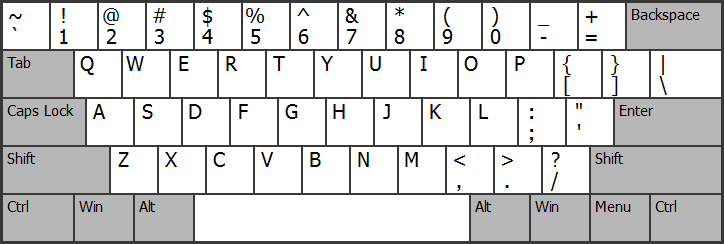
\includegraphics[scale=.8]{us_std_keyboard.png}
				\caption{Standard US Keyboard ( \url{https://kbd-intl.narod.ru/english/layouts})}
			\end{figure}
		\end{enumerate}
		%\begin{tcolorbox}[colframe=magenta, breakable, enhanced]
			\begin{proof}[\sol]
				We want to create a password system that allows for at least \(2^{128}\) (16 bytes) different passwords.
				\begin{enumerate}[(a)]
					\item We are only using lowercase letters \textcolor{red!70!black}{\texttt{a}}-\textcolor{red!70!black}{\texttt{z}}, which gives us \textbf{26} different possibilities for each character in the password. We need to solve the following equation for 
					\(n\) (the length of the password): \[
					26^n\geq 2^{128}.
					\] Then \[
					n\log(26)\geq 128\log(2)\implies n\geq\frac{128\cdot\log(2)}{\log(26)}\approx 27.2.
					\]
					\item \[
					52^n\geq 2^{128}\implies
					n\geq\frac{128\cdot\log(2)}{\log(52)}\approx 22.4.
					\]
					\item \[
					62^n\geq 2^{128}\implies n\geq\frac{128\cdot\log(2)}{\log(62)}\approx 21.5
					\]
					\item \[
					95^n\geq 2^{128}\implies n\geq\frac{128\cdot\log(2)}{\log(95)}\approx 19.5
					\]
				\end{enumerate}
			\end{proof}
		%\end{tcolorbox}
		\begin{figure}[h!]
			\centering
			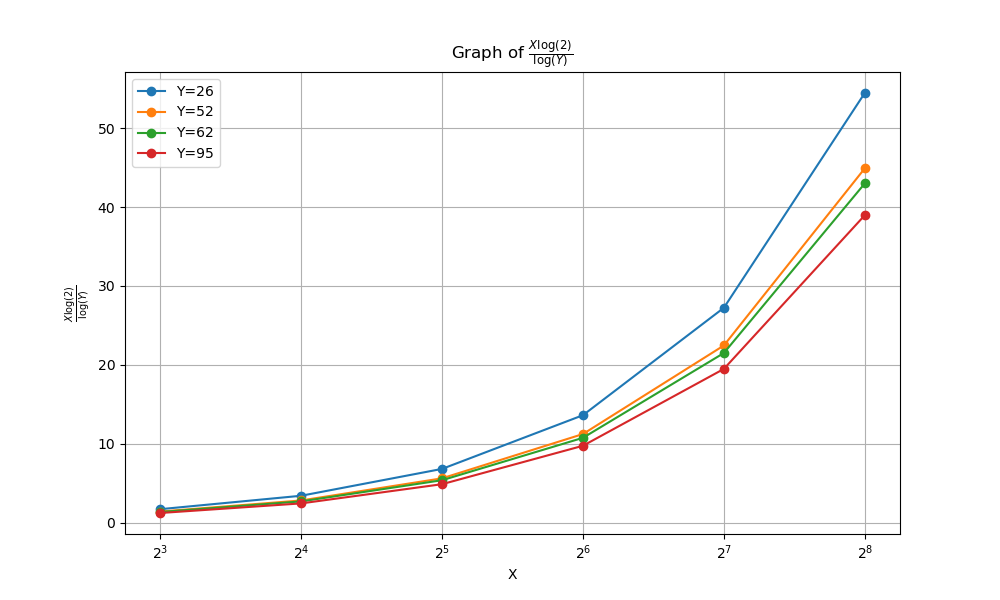
\includegraphics[scale=.75]{4_12.png}
		\end{figure}
		\begin{lstlisting}[style=sage]
import matplotlib.pyplot as plt

# Given values of X and Y
X_values = [8, 16, 32, 64, 128, 256]
Y_values = [26, 52, 62, 95]

# Initialize a plot
plt.figure(figsize=(10,6))

# Loop through each Y value
for Y in Y_values:
	# Calculate the expression for each X value
	Z = [x * log(2) / log(Y) for x in X_values]
	
	# Plot the result
	plt.plot(X_values, Z, label='Y=' + str(Y), marker='o')

# Labeling the plot
plt.title(r'Graph of $\frac{X \log(2)}{\log(Y)}$')
plt.xlabel('X')
plt.ylabel(r'$\frac{X \log(2)}{\log(Y)}$')
plt.xscale("log", base=2) # for logarithmic scale on x-axis
plt.legend()
plt.grid(True)
plt.show()
\end{lstlisting}
	\end{itemize}

	\begin{thebibliography}{9}
		\bibitem{textbook}
		M. Rosulek, \textit{The Joy of Cryptography}, [Online]. Available: \url{https://joyofcryptography.com}
	\end{thebibliography}

	% End document
\end{document}
